\chapter{Results}
\section {Waveform Morphology}
From our measurements, the results varies a lot individually. Hence, grand average and further statistical analysis won't be well-applicable. In this section, waveform morphology of the 14-channel measurements for some of the participants are shown and described.

First of all, our channels with the optode template are defined as this figure.
[picture to be added]

In the following figures. Measurements in all channels are plotted in the same scale except for the two short channels marked in thicker outlines. Channels with invalid SCI won't be taken into consideration, and hence are not shown.
\begin{figure}[H]
  \centering
    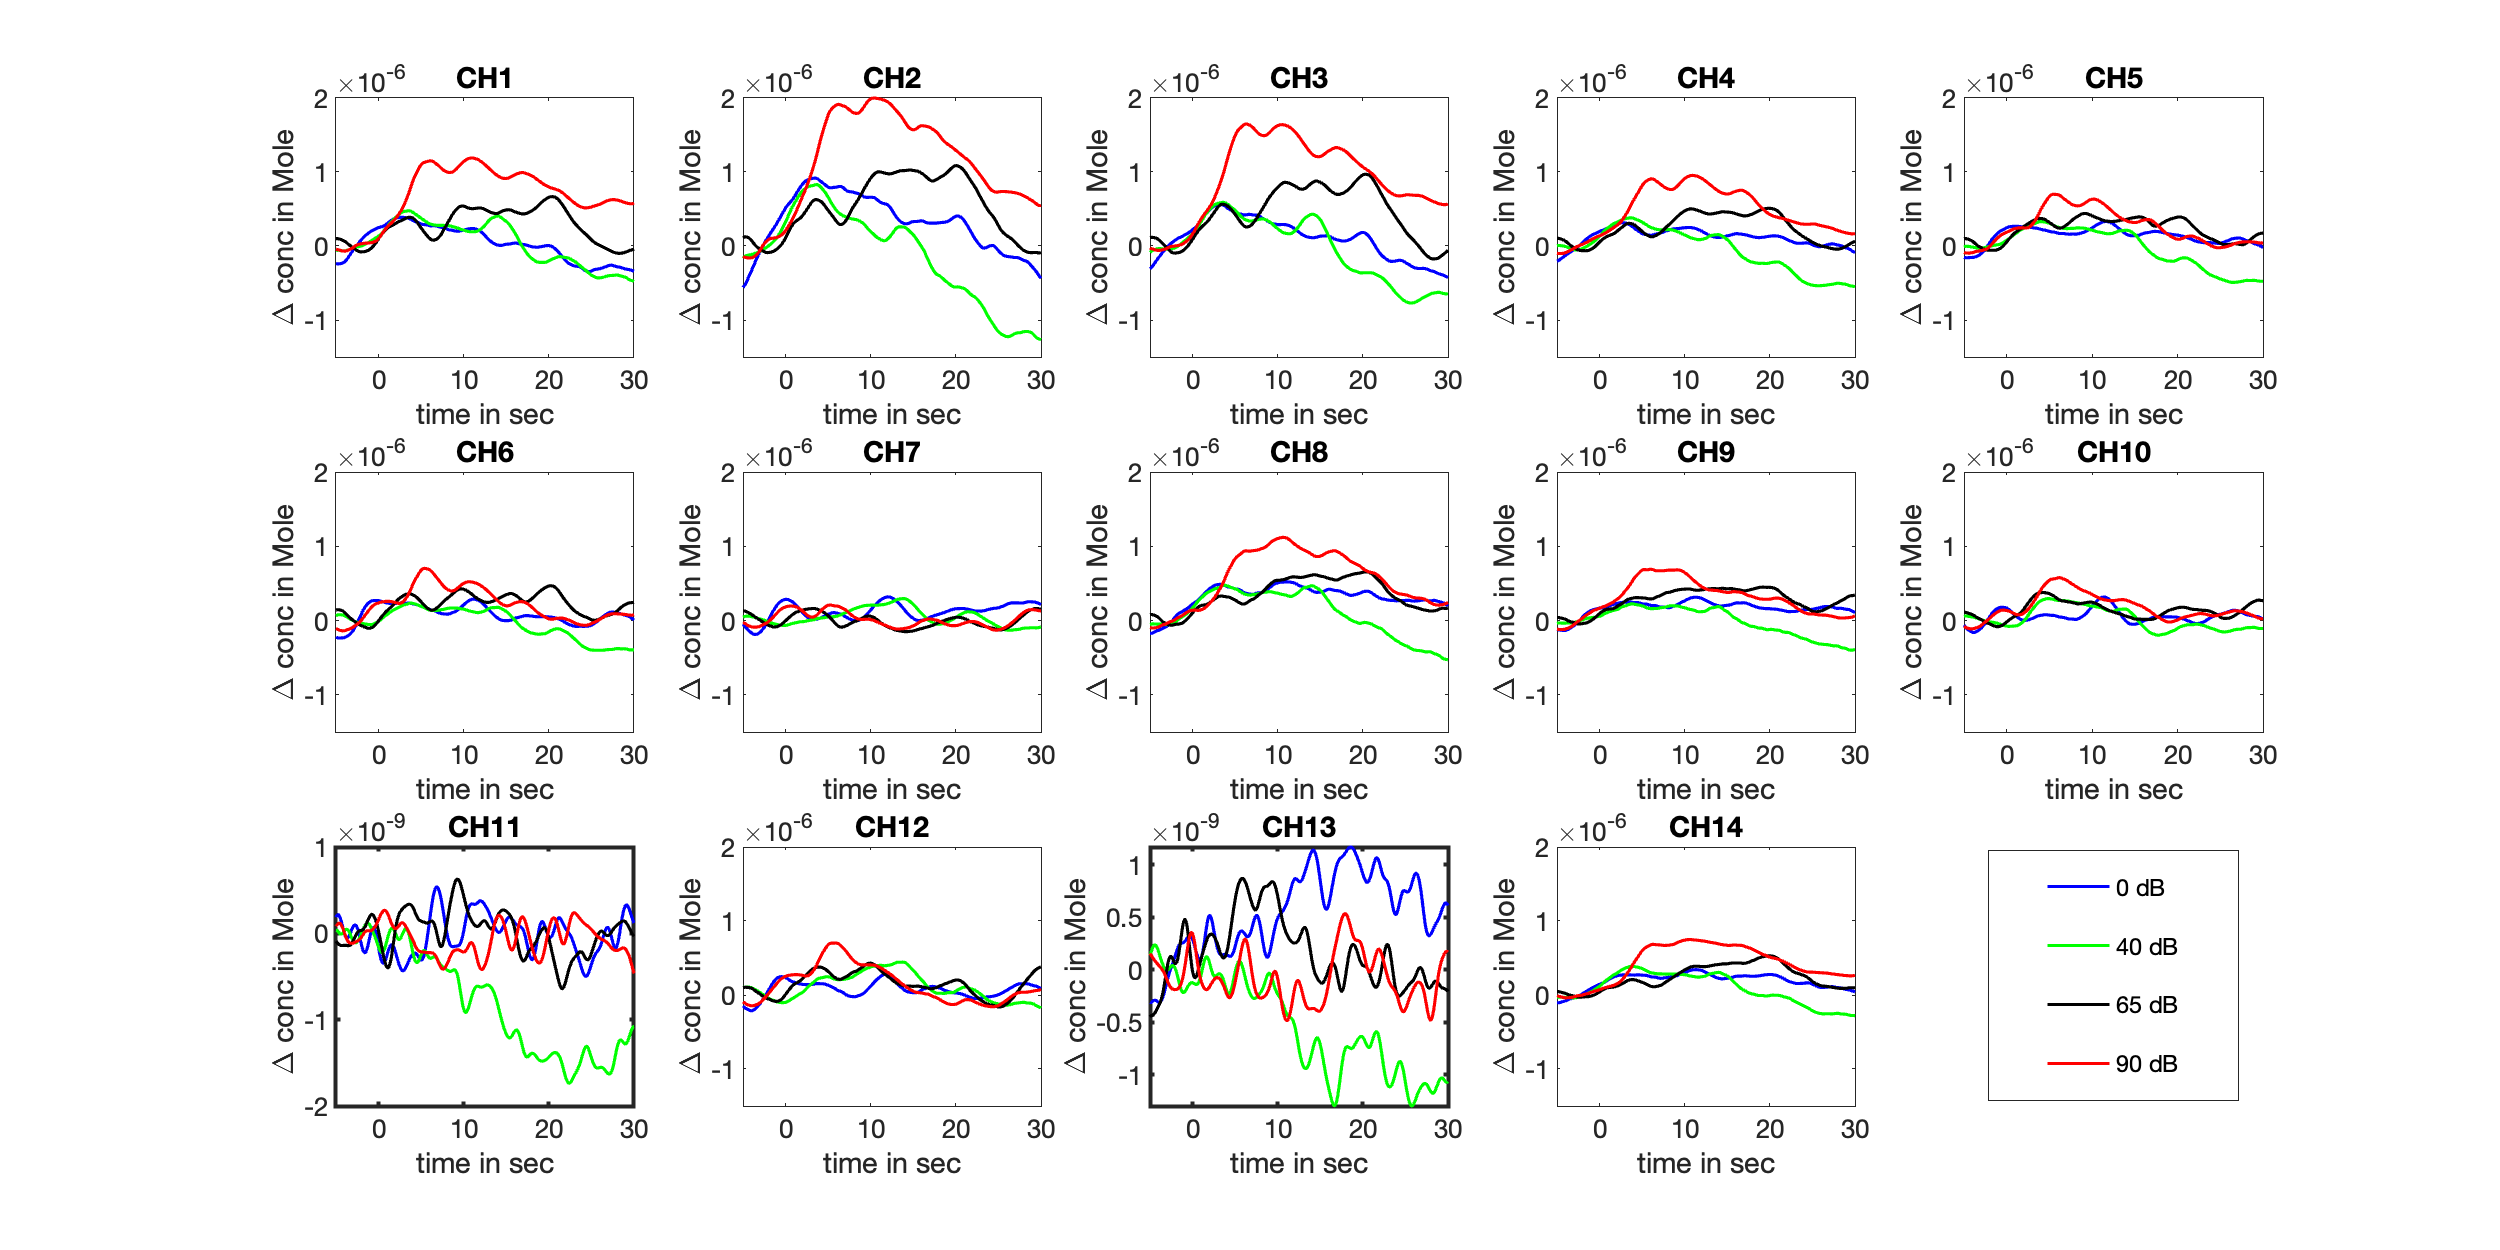
\includegraphics[scale=.4]{bilder/HbO_Mole/sub_jonas_s_HbO.png}
  \caption{Measurement from participant 3.}
  \label{fig:somesignal}
\end{figure}

\begin{figure}[H]
  \centering
    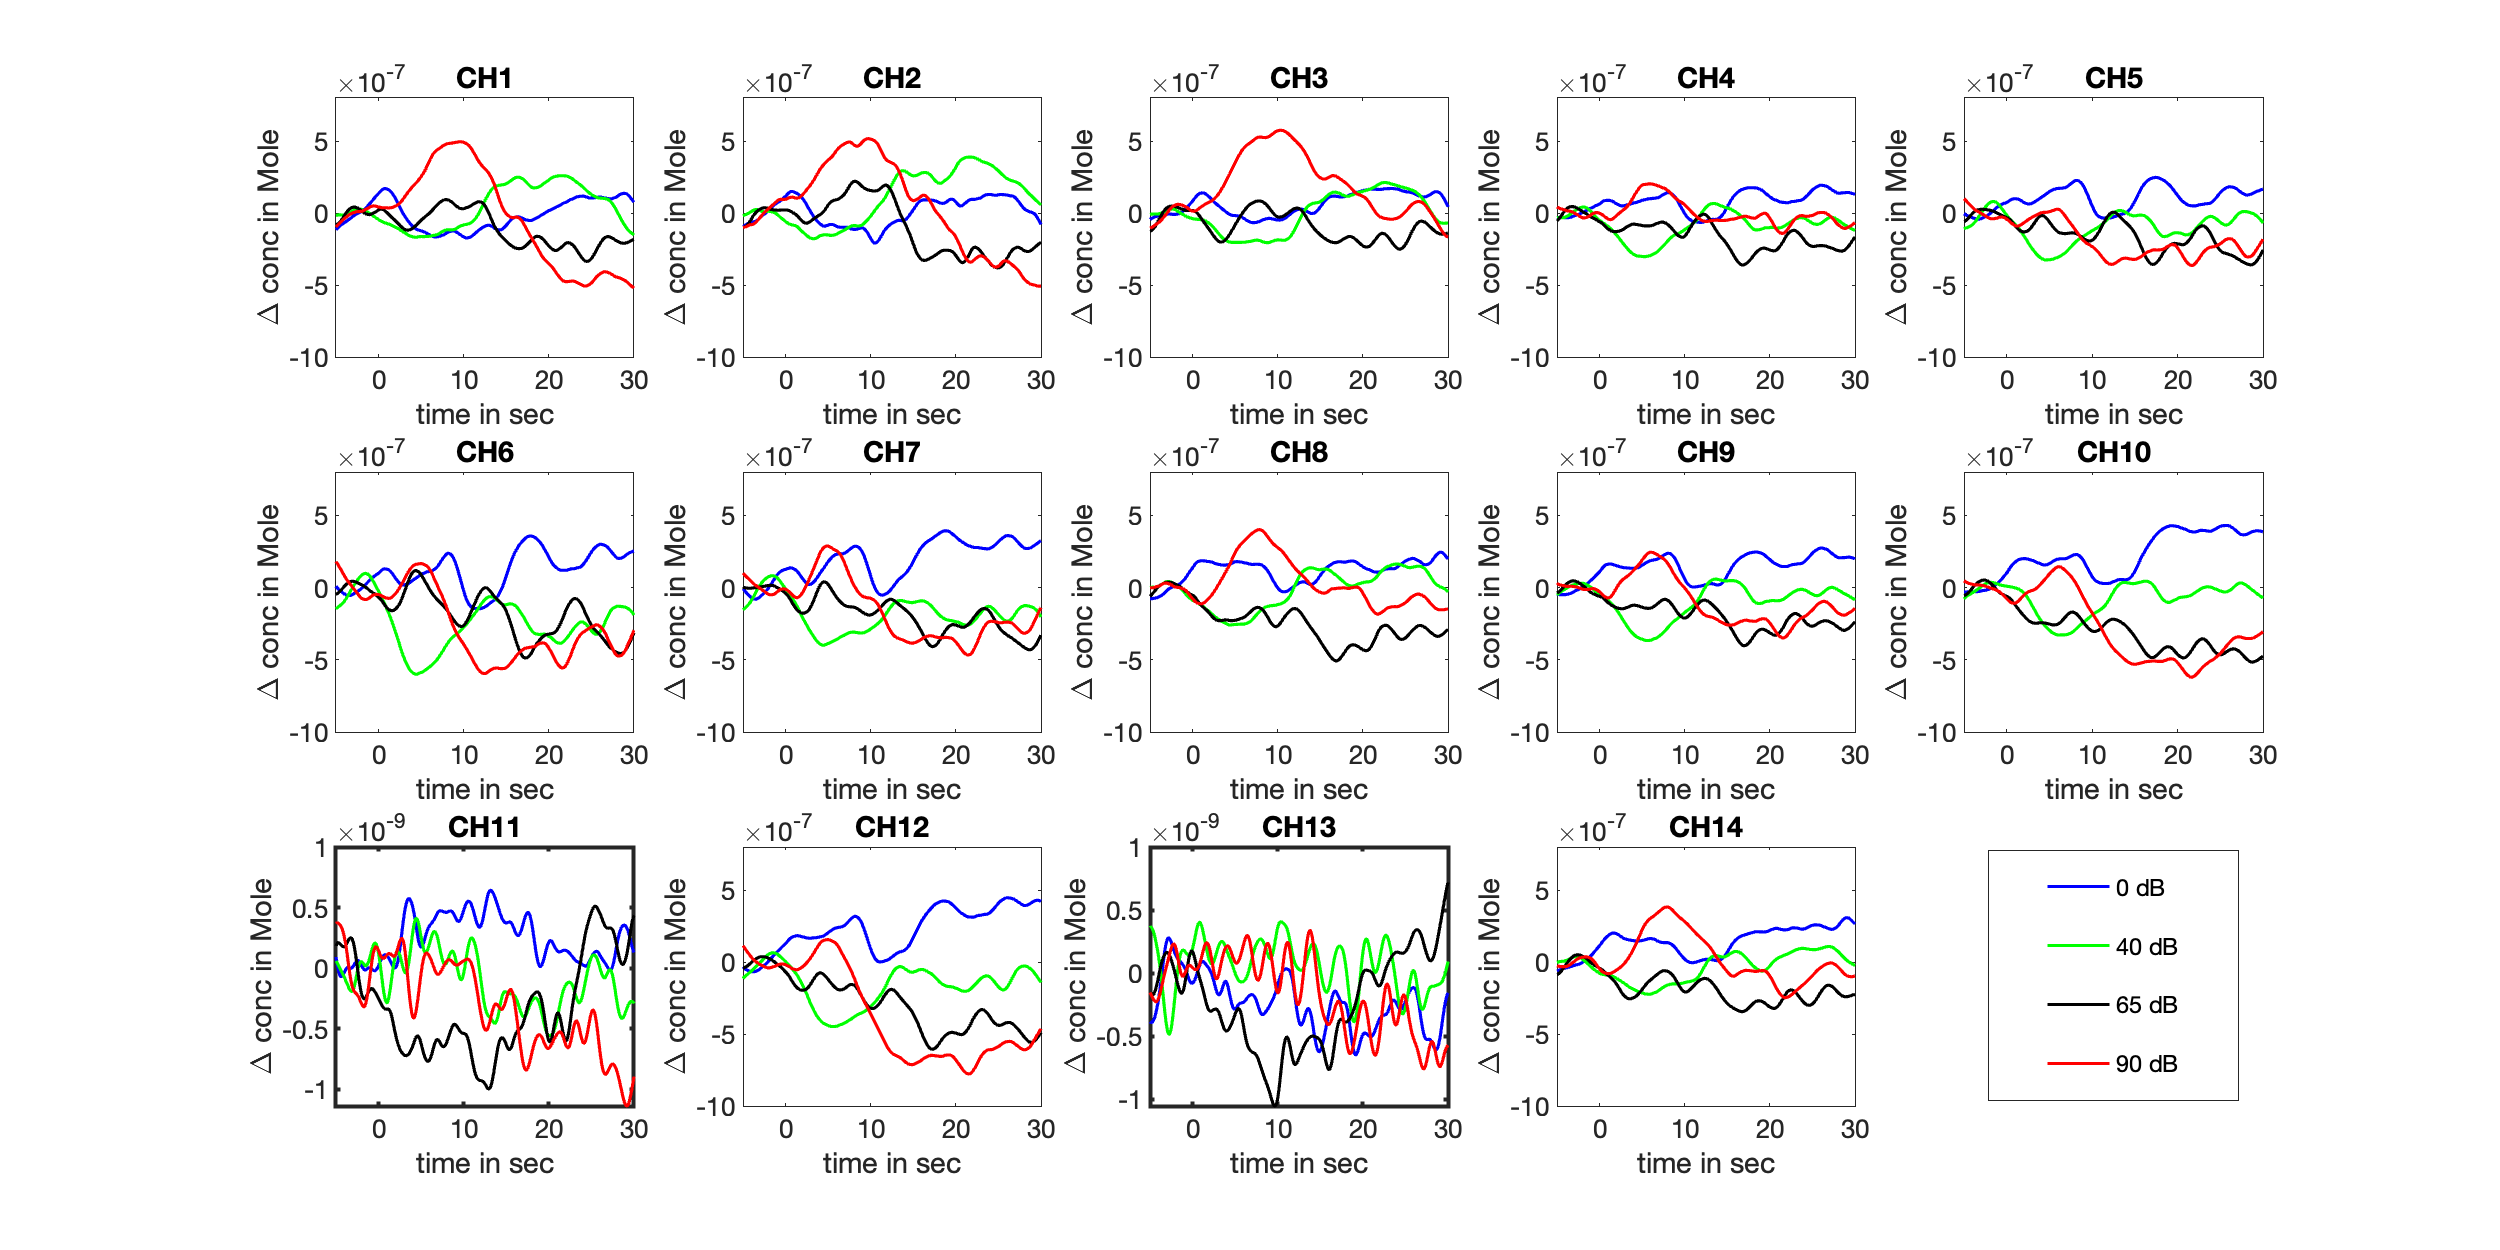
\includegraphics[scale=.4]{bilder/HbO_Mole/sub_lukas_s_HbO.png}
  \caption{Measurement from participant 5.}
  \label{fig:somesignal}
\end{figure}

\begin{figure}[H]
  \centering
    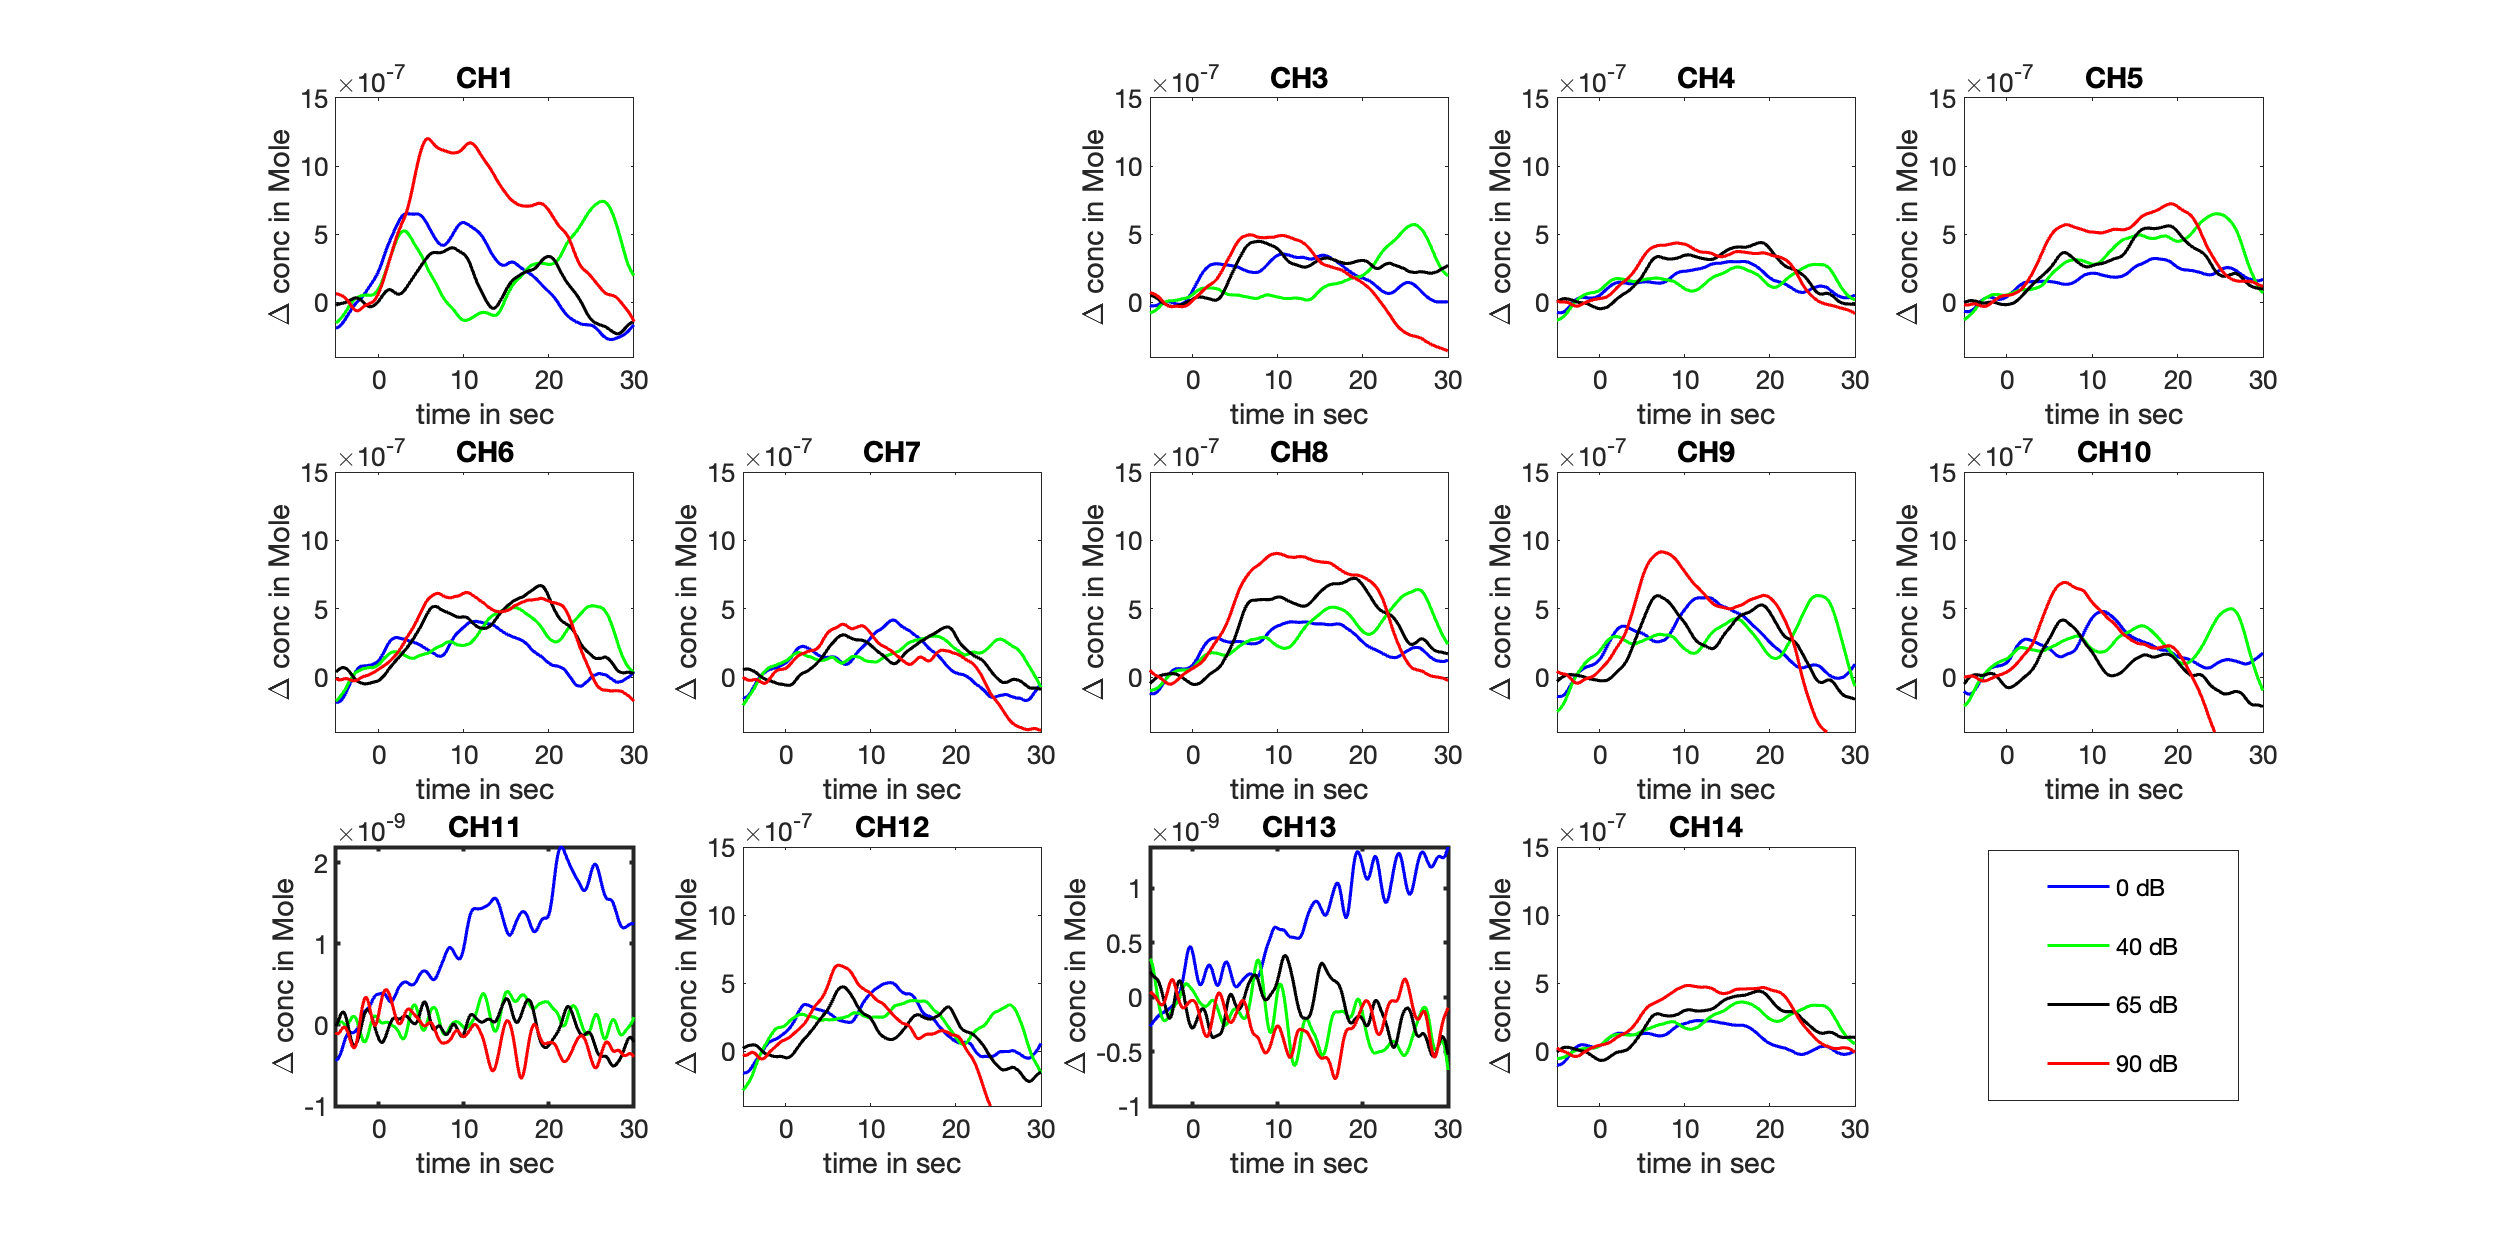
\includegraphics[scale=.4]{bilder/HbO_Mole/sub_liao_s_HbO.png}
  \caption{Measurement from participant 7.}
  \label{fig:somesignal}
\end{figure}


\begin{figure}[H]
  \centering
    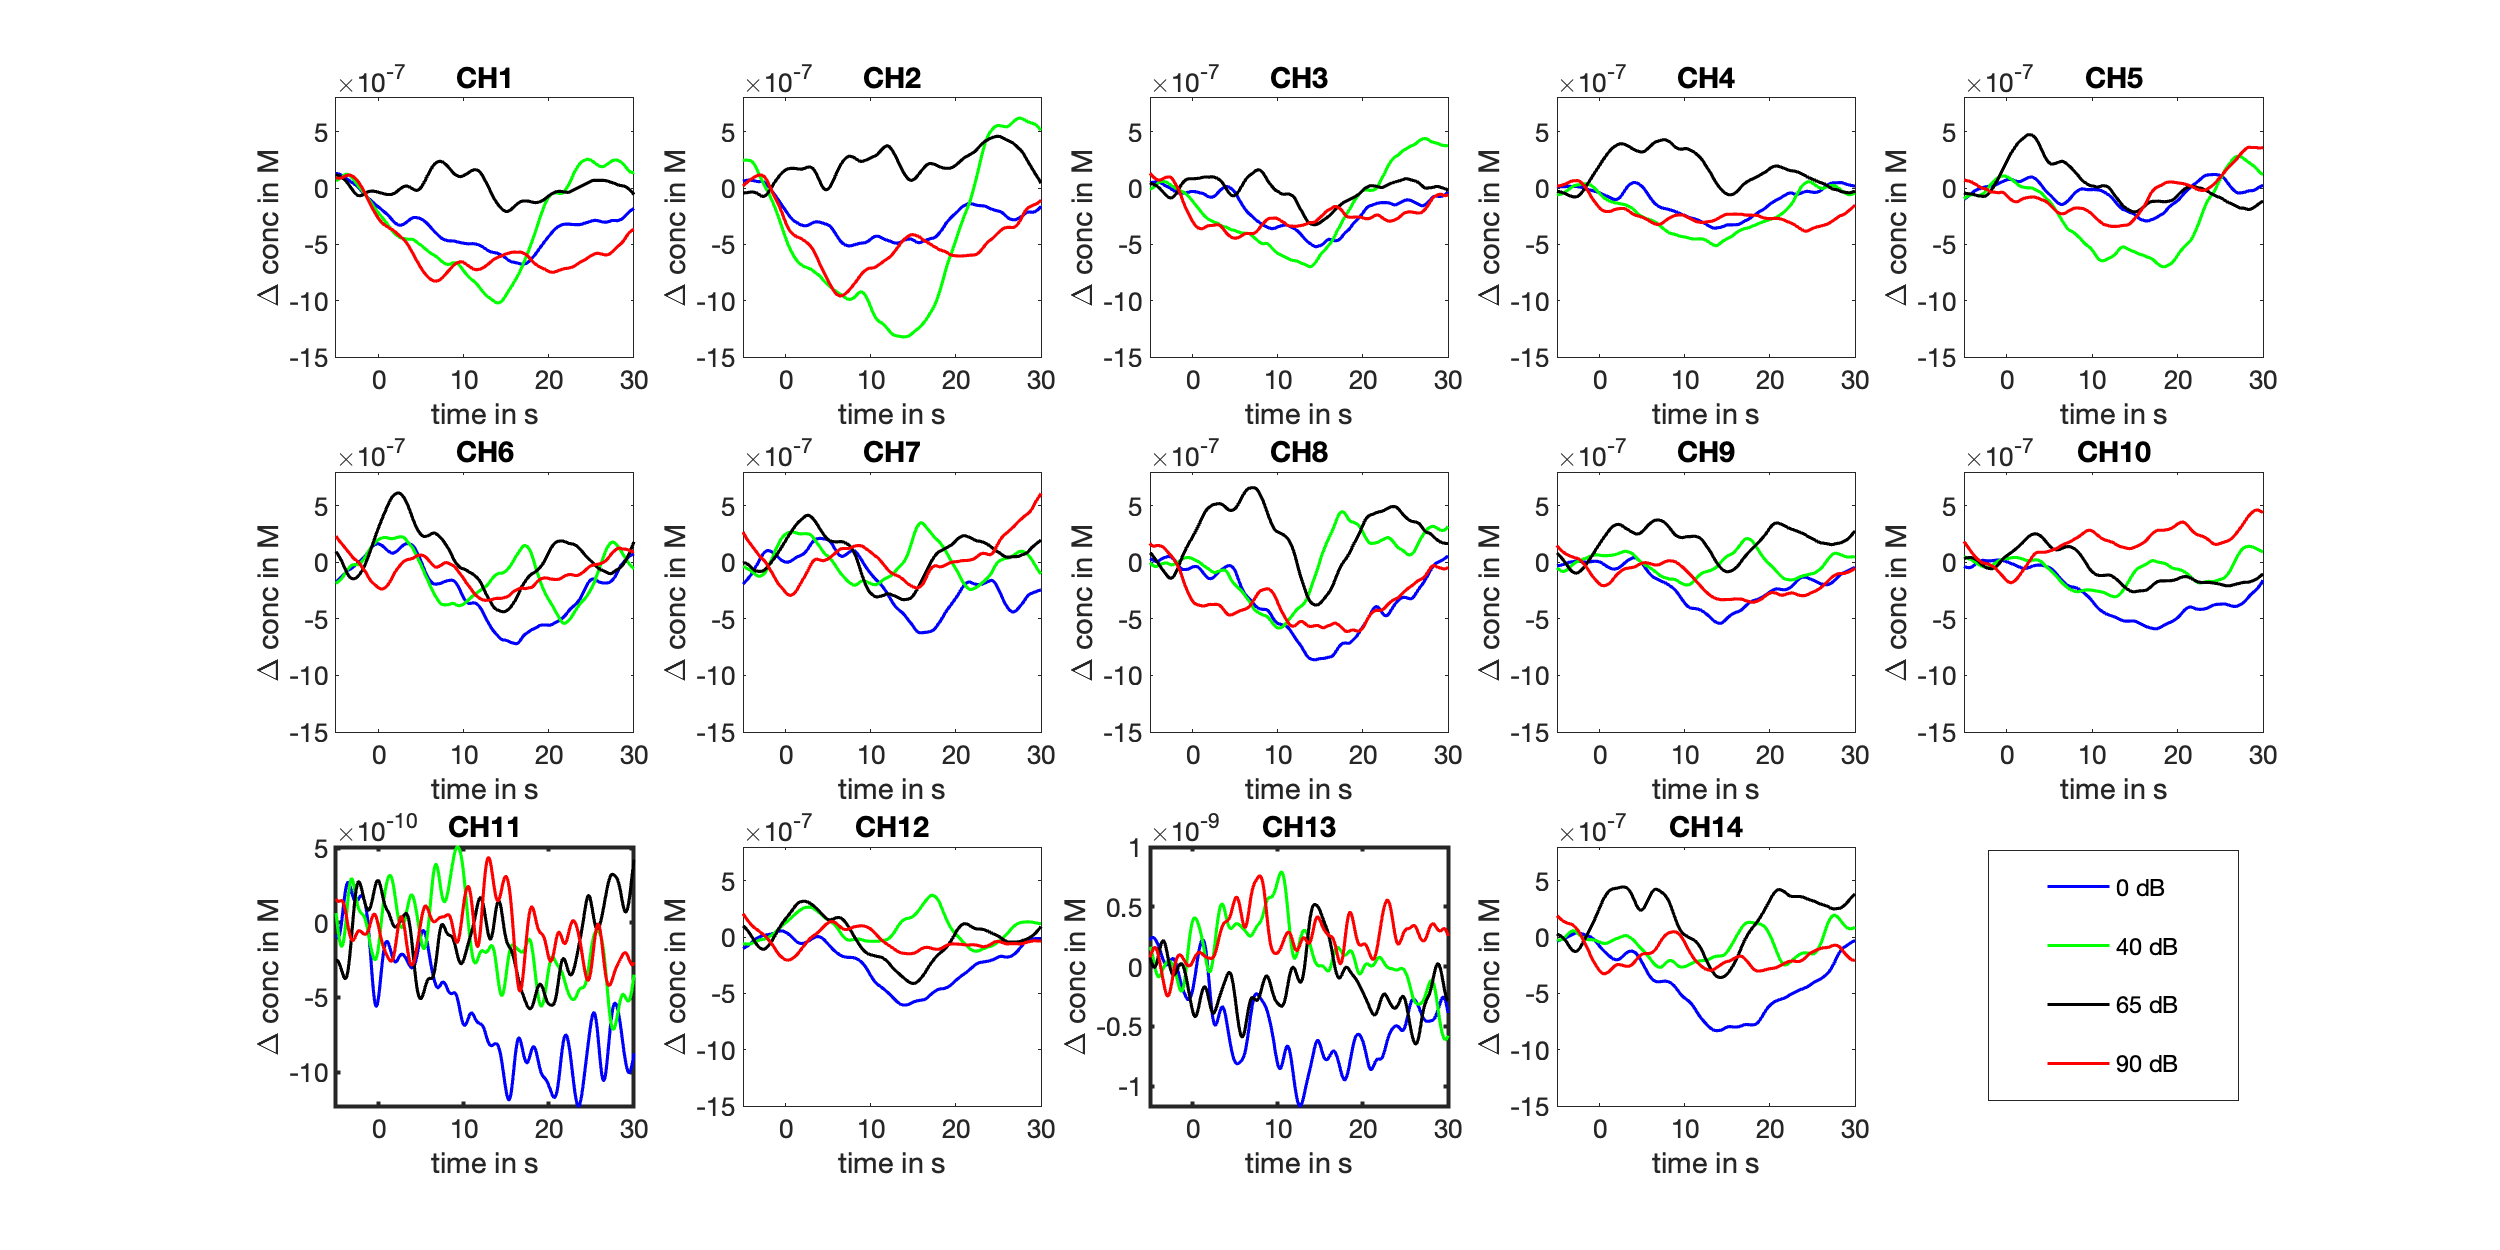
\includegraphics[scale=.4]{bilder/HbO_Mole/sub_luca2_s_HbO.png}
  \caption{Measurement from participant 8. Silent comparison}
  \label{fig:somesignal}
\end{figure}

\begin{figure}[H]
  \centering
    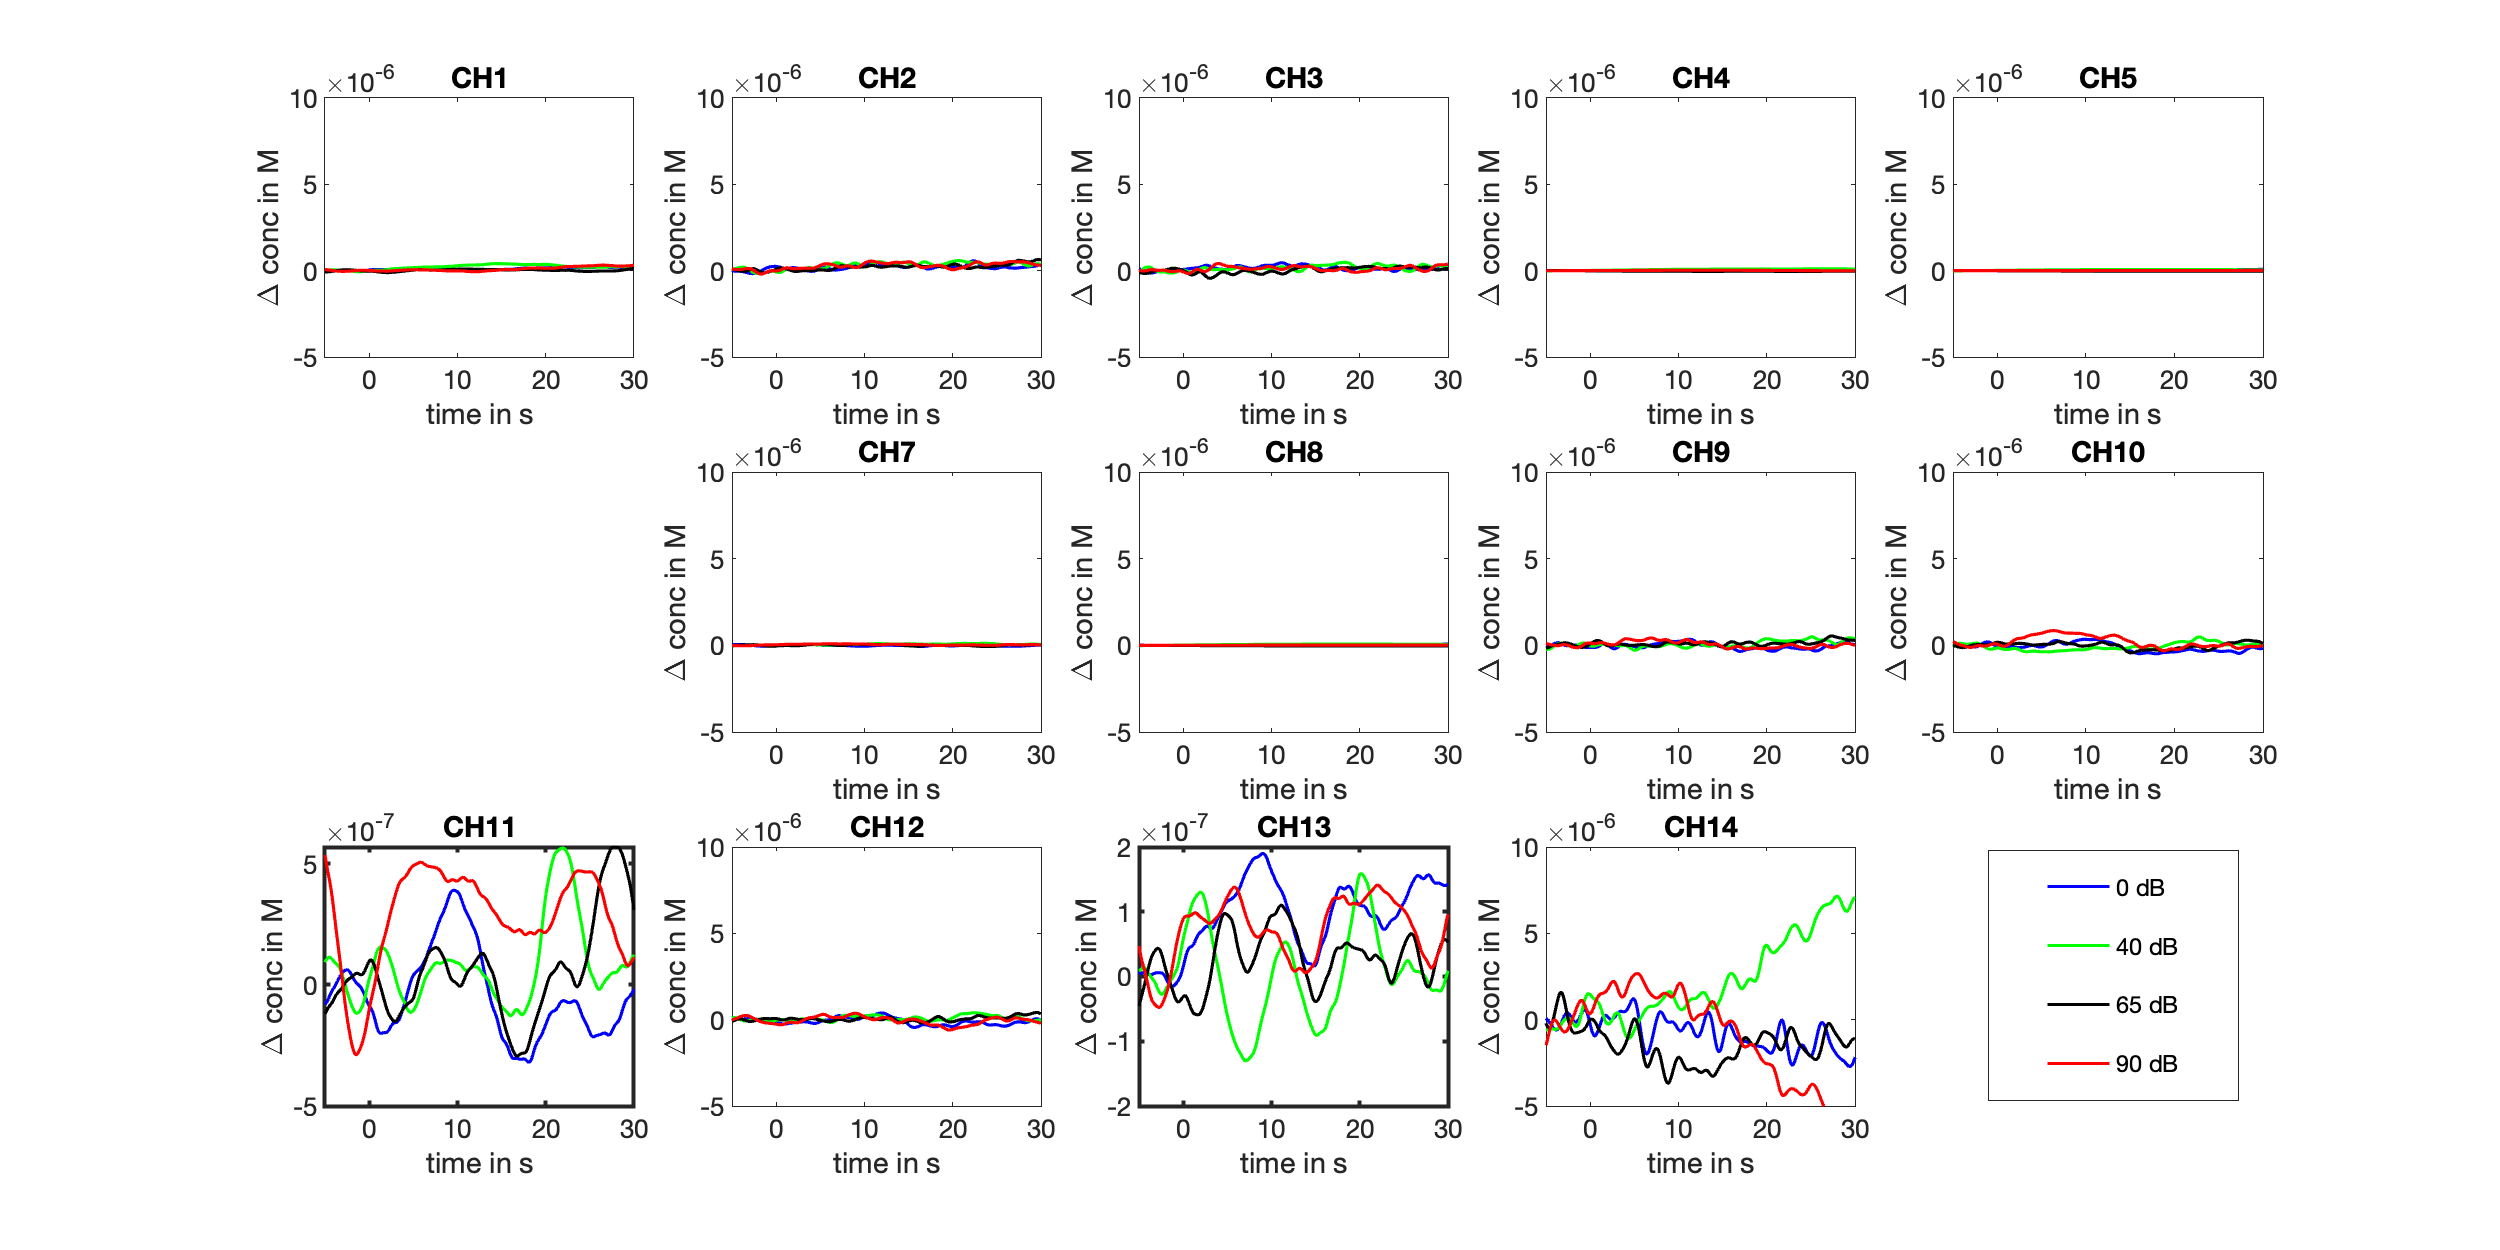
\includegraphics[scale=.4]{bilder/HbO_Mole/sub_lin_s_HbO.png}
  \caption{Measurement from participant 4.}
  \label{fig:somesignal}
\end{figure}

\newpage

\section {Regional of Interest}

\begin{figure}[H]
  \centering
    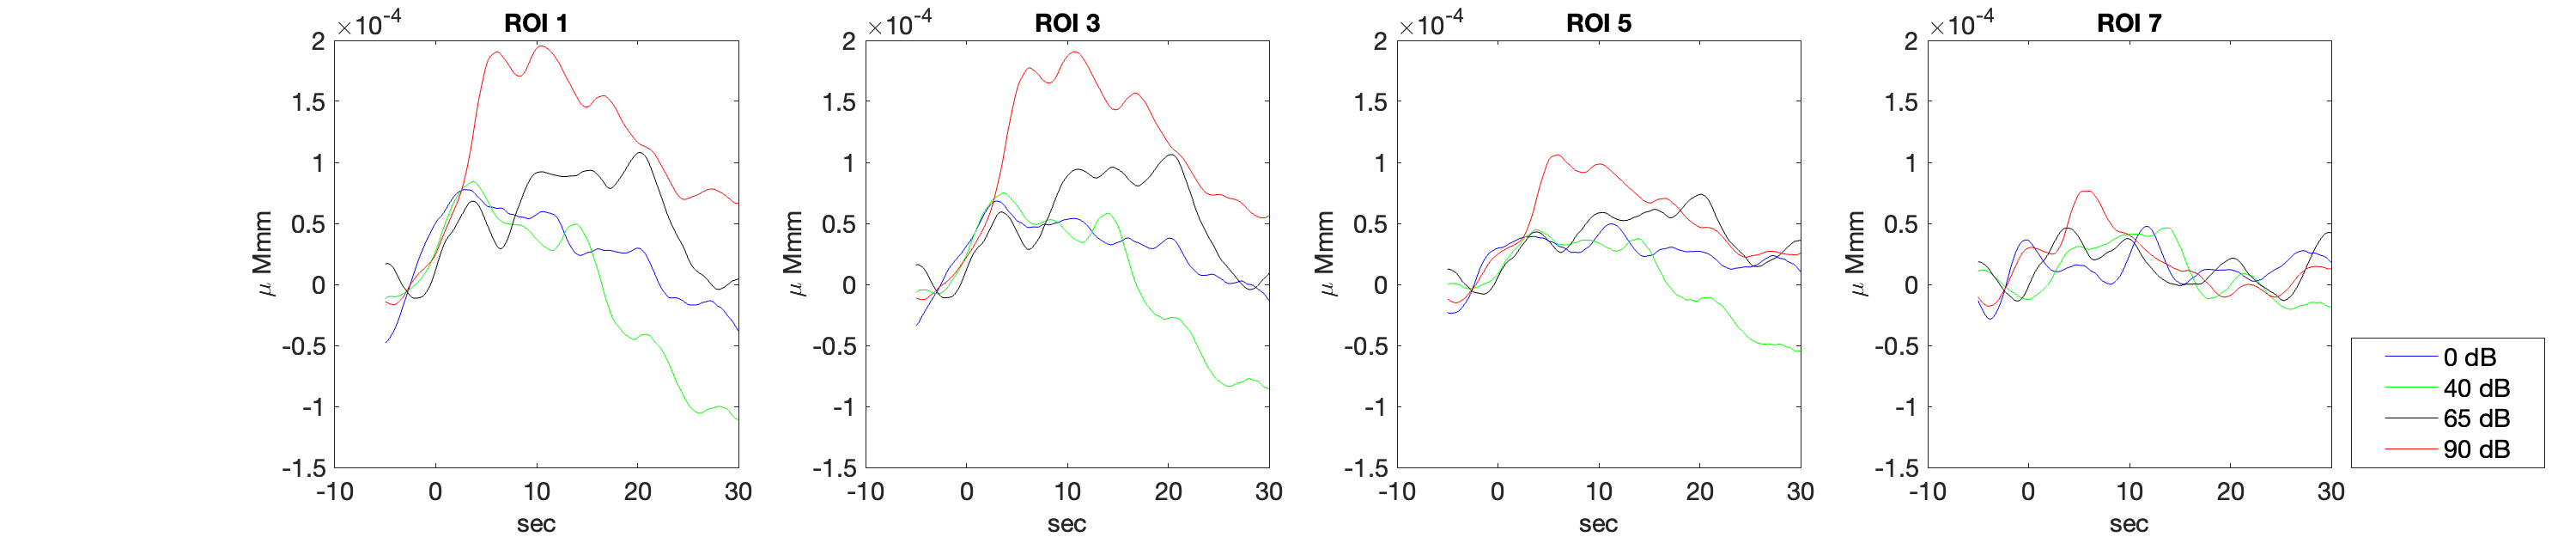
\includegraphics[scale=.3]{bilder/ROI/sub_jonas_s_HbO.png}
  \caption{Measurement from participant  3.}
  \label{fig:somesignal}
\end{figure}

\begin{figure}[H]
  \centering
    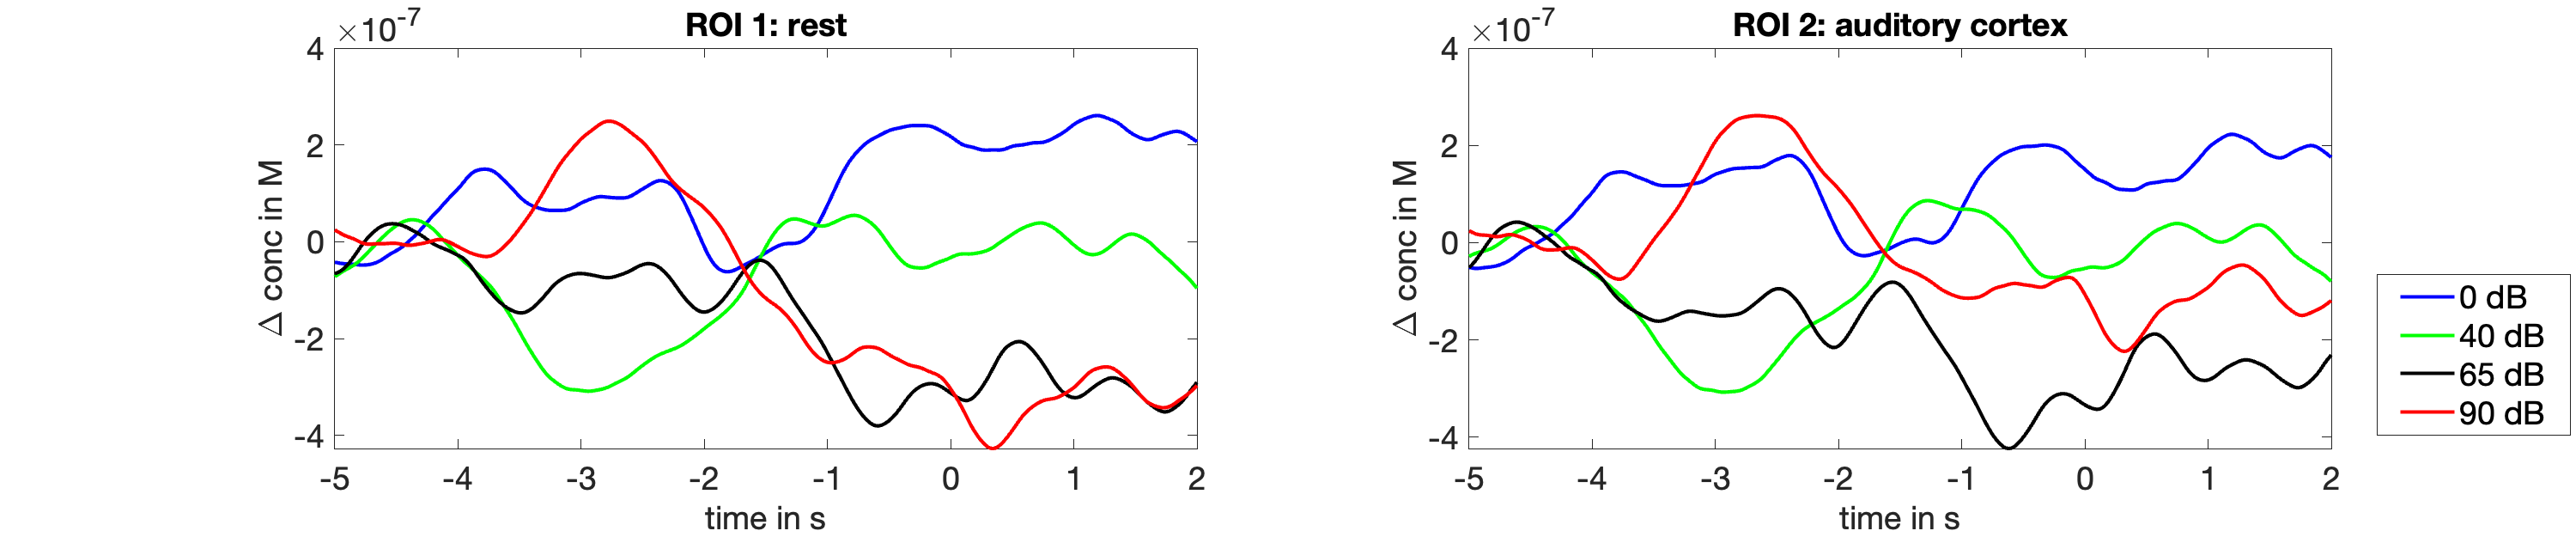
\includegraphics[scale=.3]{bilder/ROI/sub_lukas_s_HbO.png}
  \caption{Measurement from participant 4.}
  \label{fig:somesignal}
\end{figure}


\begin{figure}[H]
  \centering
    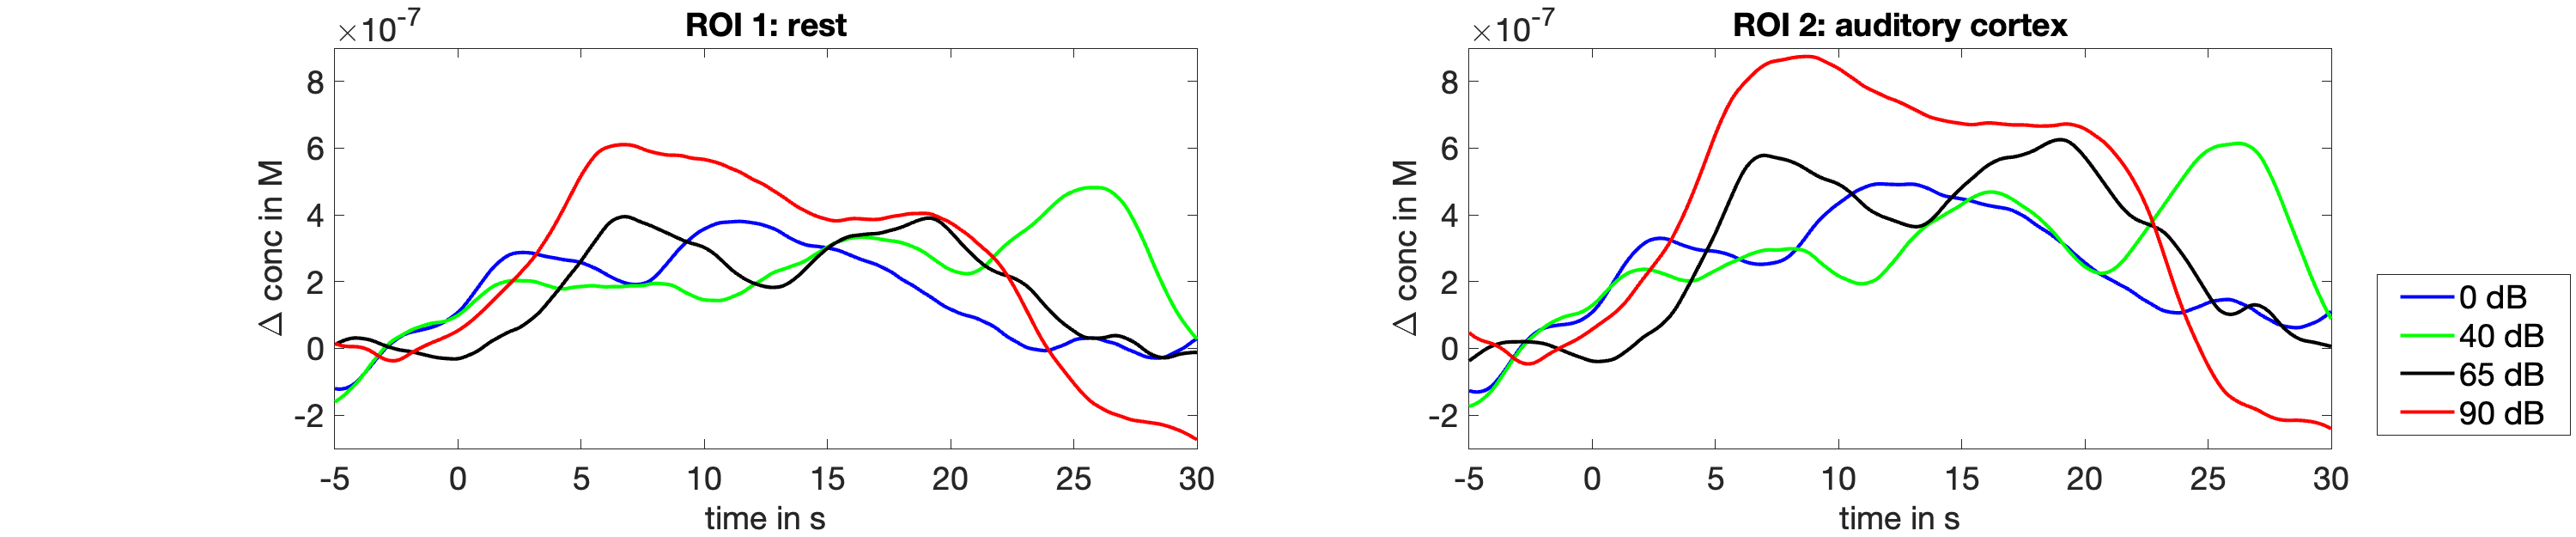
\includegraphics[scale=.3]{bilder/ROI/sub_liao_s_HbO.png}
  \caption{Measurement from participant 7.}
  \label{fig:somesignal}
\end{figure}



\begin{figure}[H]
  \centering
    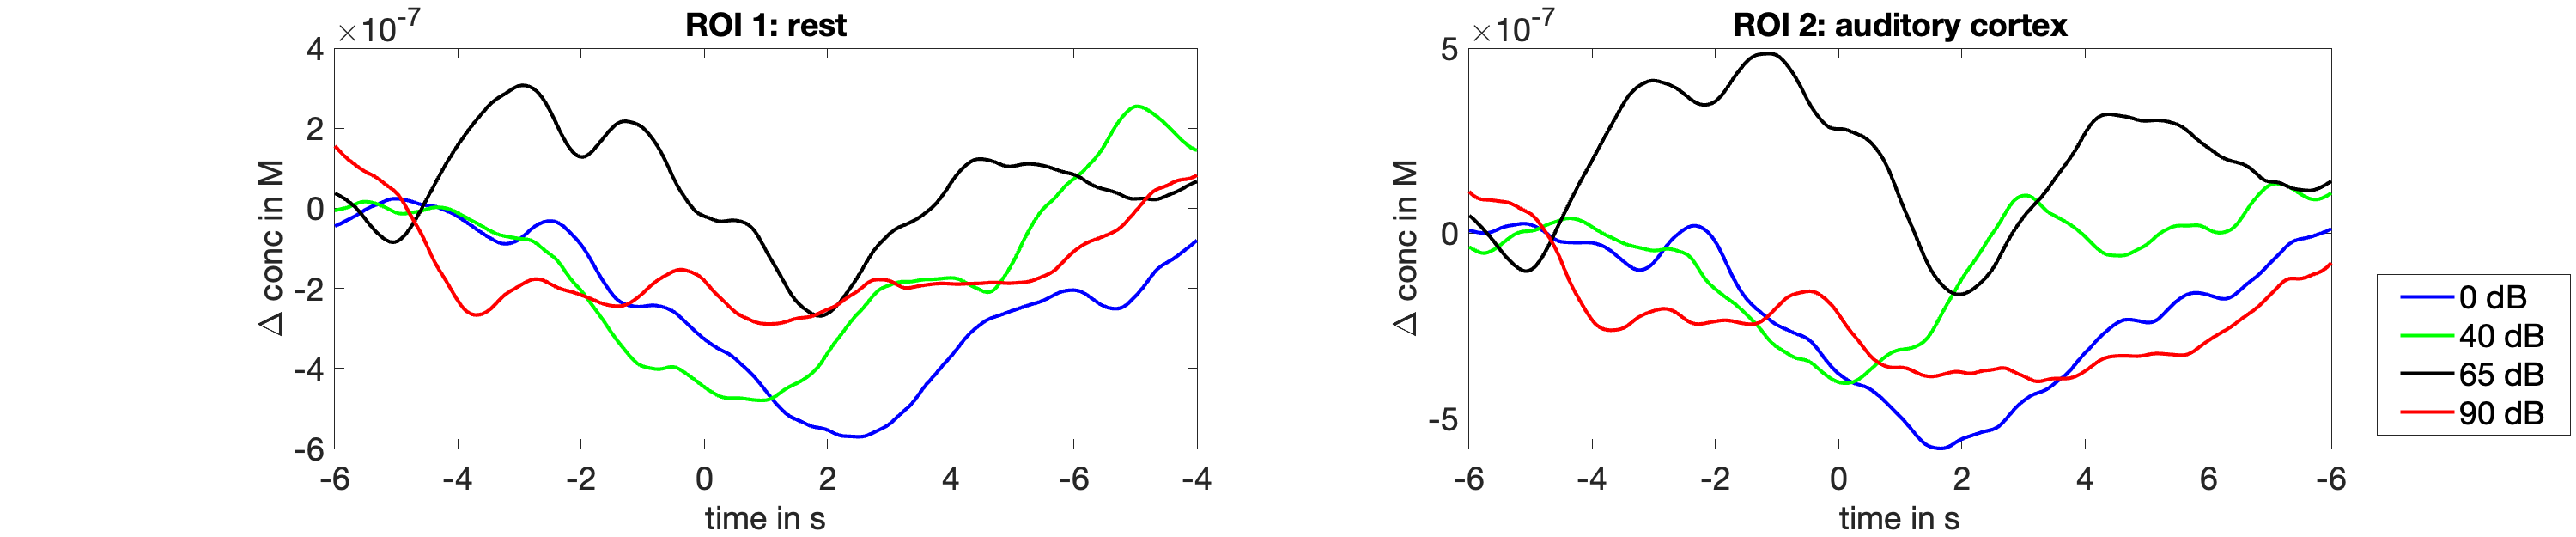
\includegraphics[scale=.3]{bilder/ROI/sub_luca2_s_HbO.png}
  \caption{Measurement from participant 8. Silent comparision.}
  \label{fig:somesignal}
\end{figure}


\begin{figure}[H]
  \centering
    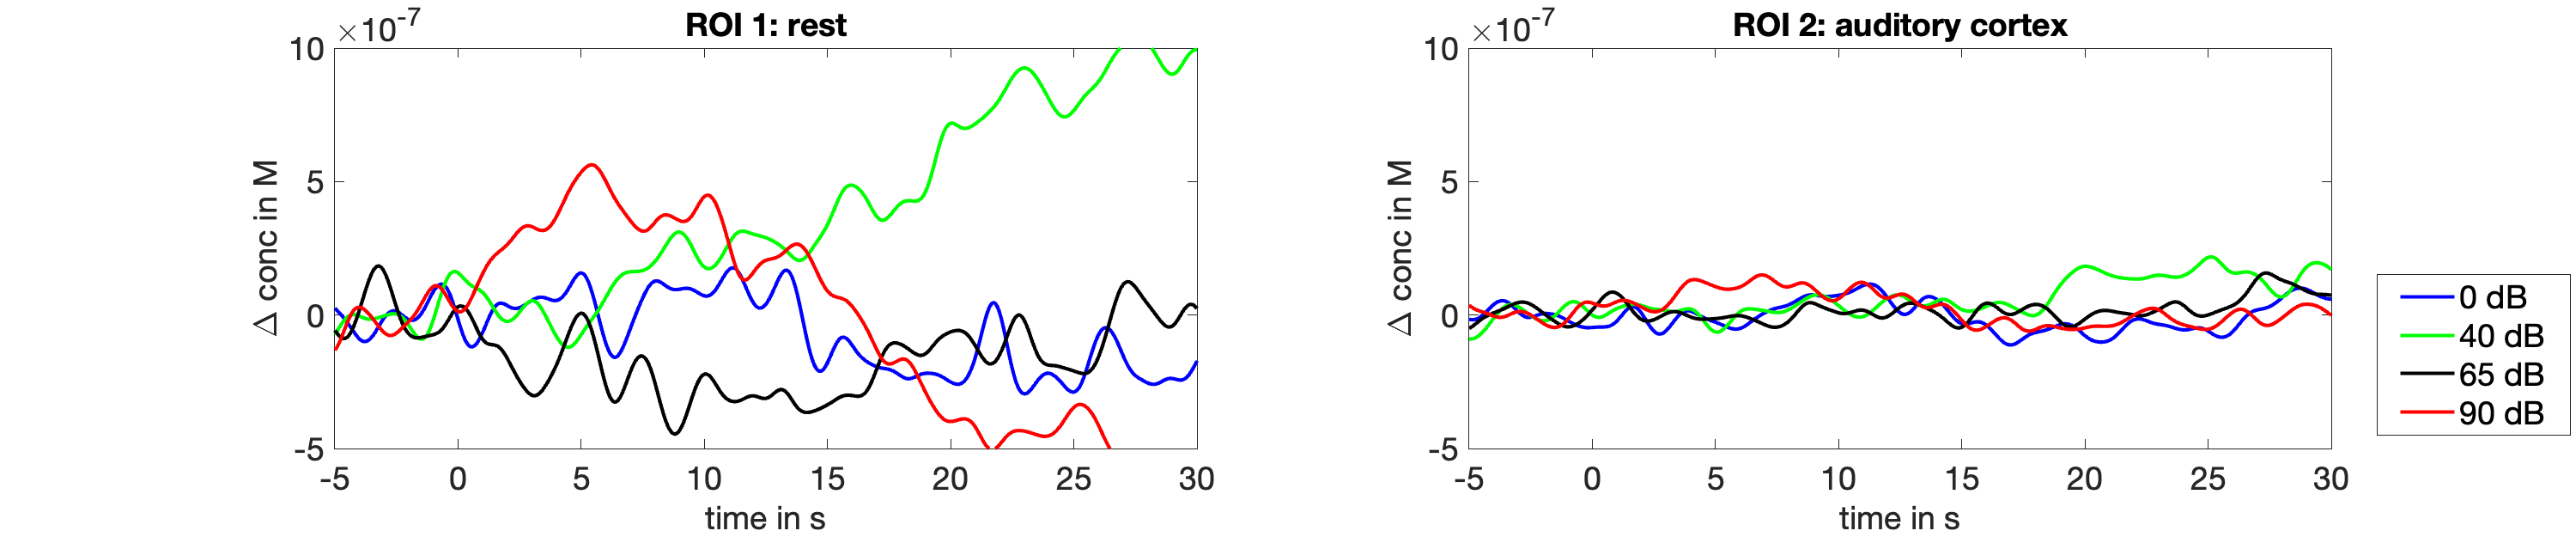
\includegraphics[scale=.3]{bilder/ROI/sub_lin_s_HbO.png}
  \caption{Measurement from participant 4.}
  \label{fig:somesignal}
\end{figure}